\chapter{Materiais e métodos}
\label{cap:exemplos}

% figuras estão no subdiretório "figuras/" dentro deste capítulo
\graphicspath{{\currfiledir/figuras/}}

%=====================================================

No início da fase de projetos foi definida uma estrutura de organização: uma adaptação do sistema \textit{waterfall} descrito em \cite{Ian19}). Apesar deste ter sido desenvolvido para projetos de software, é comum a adaptação e utilização em outros tipos de projeto. Esse sistema se forma ao alinhar, uma após a outra, as tarefas do desenvolvimento de um projeto, como mostrado na figura \ref{fig:metodologia}:

\begin{figure}[!htb]
    \centering
    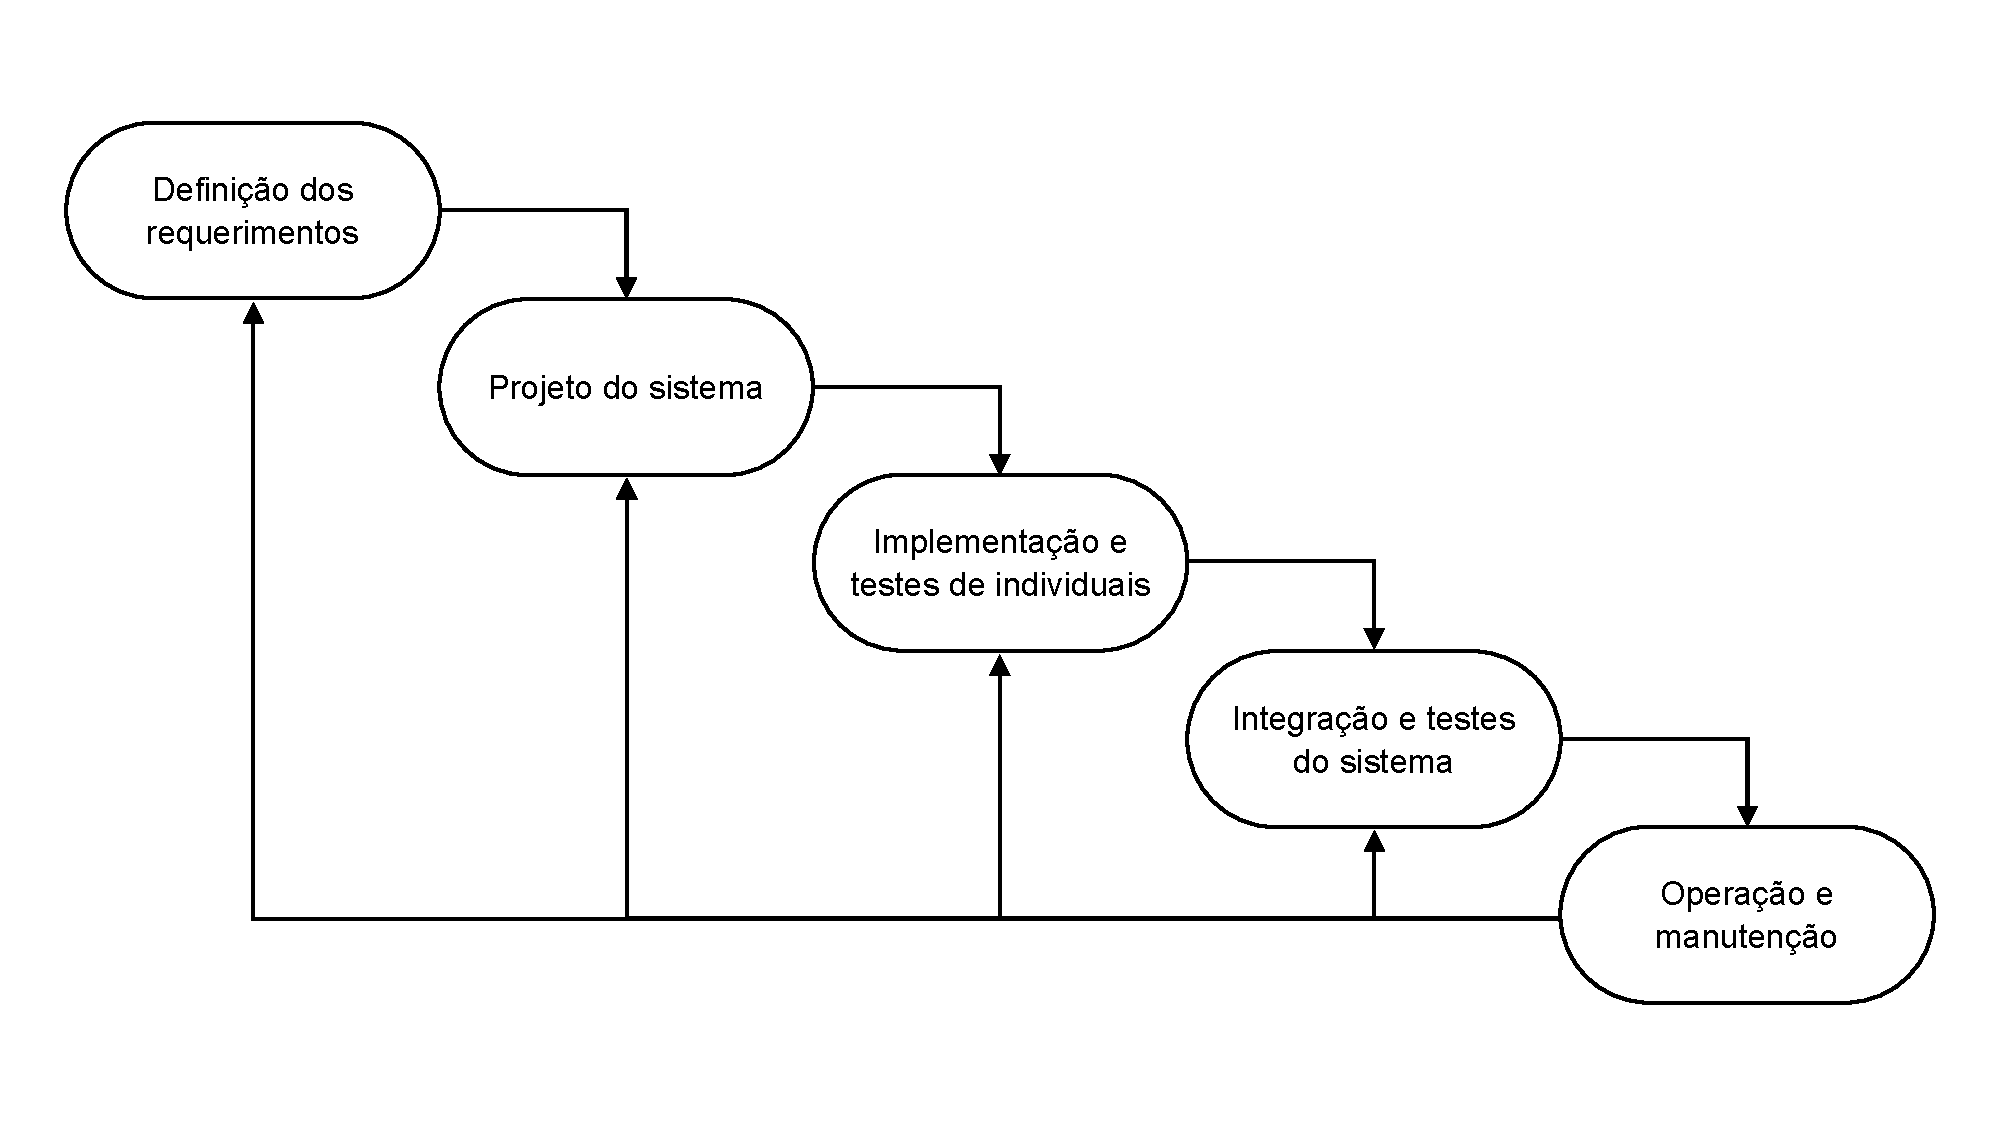
\includegraphics[width=\linewidth]{metodologia.pdf}
    \caption{Esquema das fases do projeto.}
    \label{fig:metodologia}
\end{figure}

Dentro de cada uma dessas fases de projeto diferentes atividades e documentos são desenvolvidos. A começar pela primeira etapa: definição dos requerimentos. Aqui, o processo se inicia ao criar uma lista de requerimentos, buscando responder o que é esperado do sistema projetado. A partir disso é feito um detalhamento na etapa de especificação dos requerimentos, tentando aplicar valores bem definidos como limite. Por último é feita uma validação dos requerimentos. Essa etapa gera o documento de requerimentos, que inclui a descrição dos sistemas e os requerimentos dos usuários e dos sistemas. Esse documento é usado de guia para todo o restante do projeto e a partir dele devem ser justificadas as decisões de projeto.

A próxima etapa é o desenvolvimento do projeto do sistema em si. Esse se inicia e é baseado nos documentos de entrada: o documento de requerimentos e informações dos dispositivos utilizados. A partir daí é desenvolvido o projeto de arquitetura do sistema, onde é identificada a estrutura geral do projeto e seus principais componentes, com módulos ou submódulos, como esses são distribuídos e como se relacionam. De forma mais especifica, esse relacionamento entre os módulos do é desenvolvido no projeto da interface, que descreve o relacionamento entre os componentes e com o mundo externo. E por último, é desenvolvido o projeto específico dos componentes, especificando de forma exata para que seja possível a manufatura a partir dessas especificações. Cada uma dessas atividades gera seu respectivo documento, que é utilizado como referência para cada etapa seguinte.

Com todo o projeto finalizado são desenvolvidos os testes, a começar por testes dos componentes de forma individual, após isso um teste de integração e por último, o teste completo do sistema, onde todos os requerimentos são observados e verificados se estão sendo atendidos de forma aceitável pelo sistema. Toda a documentação de planejamento de testes e os resultados deve ser desenvolvida e após isso o sistema está apto para ser utilizado pelo usuário.

Para o desenvolvimento do projeto que esse documento descreve, o sistema de armazenamento de energia foi dividido em diversos subsistemas, cada um com seus requerimentos e projetos específicos. Além disso, pelas diferenças que um projeto de sistema de armazenamento para mobilidade elétrica tem em relação à um sistema de armazenamento estacionário, alguns dos subsistemas que são empregados em veículos elétricos não estão presentes no sistema estacionário, sendo os subsistemas listados abaixo:

\begin{itemize}

    \item Veículo elétrico
    
    \begin{enumerate}
        \item Acumulador / Células
        \item Container
        \item Conexões
        \item Segmentos
        \item Plugs de manutenção
        \item HV Disconnect (HVD)
        \item Medidor de energia
        \item Fusíveis
        \item Fusível principal
        \item Relés de isolamento do acumulador (AIRs)
        \item Indicador LED do acumulador
        \item Circuito de pré-carga
        \item Circuito de descarga
        \item Circuito Shutdown
        \item Placas de circuito impresso (PCBs)
        \item Sistema de gerenciamento do acumulador (AMS)
        \item Dispositivo de monitoramento do isolamento (IMD)
        \item Carregador
        \item Circuito Shutdown do carregador
    \end{enumerate}

    \item Microrrede
    
    \begin{enumerate}
        \item Acumulador / Células
        \item Container
        \item Conexões
        \item Plugs de manutenção
        \item Fusíveis
        \item Fusível principal
        \item Relés de isolamento do acumulador (AIRs)
        \item Circuito de pré-carga
        \item Circuito de descarga
        \item Circuito Shutdown
        \item Placas de circuito impresso (PCBs)
        \item Sistema de gerenciamento do acumulador (AMS)
    \end{enumerate}
    
\end{itemize}





